\documentclass[10pt,a4paper]{scrartcl}
\usepackage[utf8x]{inputenc}
\usepackage{ucs}
\usepackage{amsmath}
\usepackage{amsfonts}
\usepackage{amssymb}
\usepackage{ngerman}
\usepackage{graphicx}
%\usepackage{luximono}
%\usepackage[T1]{fontenc}
\begin{document}
\section*{Assignment 1}
\subsection*{Exercise 1: OSI model}
\begin{itemize}
\item \textbf{Application} (Anwendungsschicht): z.B. virtual terminals, Dateiübertragungen (wegen unterschiedlicher Dateisysteme) [FTP, SMTP, HTTP, SSH...]
\item \textbf{Presentation} (Darstellungsschicht): Syntax und Semantik. Datensätze beispielsweise müssen abstrakt repräsentiert werden, weil ihre Einträge auf unterschiedlichen Computer u.U. unterschiedlich codiert werden (ASCII, Unicode...) 
\item \textbf{Session} (Kommunikationssteuerungsschicht): Dialogsteuerung (token management, synchronization, checkpoints in datenübertragung) 
\item \textbf{Transport} (Transportschicht): nimmt Daten der Session Layer entgegen, portioniert sie, gibt sie an die Network Layer weiter und guckt ob alles klappt. Stauvermeidung. Einheitlicher Zugriff für die überliegenden Schichten, damit die sich nicht um den Hardwarekram kümmern müssen. [TCP, UDP]
\item \textbf{Network} (Vermittlungsschicht): Paketweiterleitung, Stauvermeidung, Vermeidung von Schwierigkeiten bei der Verbindung von verschiedenen Netzwerken (Unterschiede in Adressierung, Paketgrößen...) [IP, ICPM]
\item \textbf{Data Link} (Sicherungsschicht): Macht Frames, verschickt die, wartet auf Acknowledgement Frames, erstellt Prüfsummen, ermöglicht Flußkontrolle, also die empfangende Seite regelt die Geschwindigkeit der Übertragung, Piggybacking [IEEE 802.11, Ethernet, ARP]
\begin{itemize}
\item LLC (Logical Link Control)
\item MAC (Media Access Control)
\end{itemize}
\item \textbf{Physical} (Bitübertragungsschicht): Wieviel Volt drückt 1 aus, wielange dauert ein Bit, Wie wird die Verbindung hergestellt? Elektrisch, mechanisch.
\end{itemize}


\subsection*{Exercise 2: Path Selection}
Die Pfade die ein Paket zu nehmen hat werden in der Netzwerkschicht gewählt (Routing)

\subsection*{Exercise 3: Physical Layer}
Bitübertragungsschicht definiert, welche Spannung ein 1-Bit darstellt und welche ein 0-Bit, wie lange diese Spannung aufrechterhalten wird, über welches Medium übertragen wird und die physikalische Datenrate.

\subsection*{Exercise 4: Casting Information}
\begin{itemize}
\item \textbf{unicast}: Punkt-zu-Punkt Verbindung, Sender kennt Adresse des Empfängers. Beispiel: Webserveranfrage
\item \textbf{multicast}: Es wird gleichzeitig an alle Empfänger gesendet, die sich dafür eingetragen haben. Die Pakete werden erst auf den Routern vervielfältigt, dadurch wird an der Quelle Bandbreite gespart und die Quelle muß die einzelnen Empfänger nicht kennen. Beispiel: Videosteaming
\item \textbf{broadcast}: Es wird an alle Adressen in einem bestimmten Adressraum gesendet, also zum Beispiel alle Computer in einem Netzwerk. Wireless ist physikalisch gesehen immer Broadcast. Beispiel: ARP
\item \textbf{concast}: Inverse Multicast
\item \textbf{Anycast}: Gesendet wird zum jeweils besten Emfänger. Beispiel: DNS
\end{itemize}

\subsection*{Exercise 5: Overhead}
\begin{itemize}
\item connection-oriented: wie Telefon, man ruft an, es geht wer ran, man überträgt Daten, man legt wieder auf. Die Verbindung funktioniert also wie eine Röhre. Daß die Daten ankommen, ist garantiert.
\item connectionless: wie die Post. Auch wenn man mehrere Briefe an dieselbe Adresse schickt, können die jeweils ganz verschiedene Wege nehmen. Die können auch in einer ganz anderen Reihenfolge ankommen. 
\end{itemize}
Connection-orientierte Verbindungen haben mehr Overhead. Die Verbindung muß ja erst hergestellt werden und wieder abgebrochen, außerdem gibt es Flußkontrolle und Stauvermeidung.

\subsection*{Exercise 6: Services in a layered communication system}
\begin{enumerate}
\item Dafür, daß in einem Schichtenmodell alle Schichten nur mit denen direkt unter oder über ihnen sprechen dürfen, spricht, daß das die Austauschbarkeit von den Implementierungen der Schichten erleichtert. Außerdem erhöht es die Sicherheit.
\item Alternative: Cross-Layering????
\end{enumerate}

\subsection*{Exercise 7: Latency and bandwidth}
Latency ist die Verzögerung, die zu einer nicht unterschreitbaren Übertragungszeit führt. Sie wird durch Endgeräte wie Modems hervorgerufen. In Ethernets ist sie ziemlich gering.
\begin{enumerate}
\item \textbf{FTP}: Weil große Dateien übertragen werden, ist bandwidth wichtiger
\item \textbf{SSH}: Daten werden verschlüsselt, müssen aber schnell ankommen, also ist beides wichtig. bei scp eher bandwidth
\item \textbf{Pay-TV Video Streaming}: Es werden große Datenmengen übertragen. bandwidth ist wichtiger
\item \textbf{Remote controlled emergency shut-off system}: weil das emergeny drinsteckt, muß es bestimmt schnell gehen. latency
\item \textbf{Telemedicine in the surgery}: high resolution, update in real time. beides
\item \textbf{Access to the www}: Beides. 
\item \textbf{E-Mail}: Beides
\end{enumerate}

\subsection*{Exercise 8: Asynchronous vs. synchronous transmission}
\begin{itemize}
\item Synchrone Übertragung:
\begin{list}{}{}
\item - aufwendig zu implementieren
\item + geringer overhead, höhere effizienz, weniger kontrollzeichen nötig
\end{list}
\item Asynchrone Übertragung:
\begin{list}{}{}
\item - großer overhead wegen start- und stopbits
\item + einfach zu implementieren
\end{list}
\end{itemize}

\subsection*{Exercise 9: Connection Properties}
\begin{itemize}
\item \textbf{simplex}: Daten werden nur in eine Richtung übertragen [pager]
\item \textbf{duplex}: Daten werden gleichzeitig in beide Richtungen übertragen [ethernet, telefon]
\item \textbf{half-duplex}: Daten werden abwechselnd in beide Richtungen übertragen [walkie-talkie]
\end{itemize}

\subsection*{Exercise 10: Terminology}
\begin{itemize}
\item Signal: Physikalische Codierung von Daten
\item Data: Repräsentationen von Informationen. Müssen zur Übertragung in Signale umgewandelt werden
\item Information: Daten die durch Menschen interpretiert werden. 
\end{itemize}

\subsection*{Exercise 11: Networks in the Real World}
Ethernet, WLAN, GSM, UMTS...

\subsection*{Exercise 12: The core of the Internet}

\section*{Assignment 2}

\subsection*{Exercise 1: Required Reading: IETF}
RFC 2026 Internet Engineering Task Force

\subsection*{Exercise 2: Reference Models}
Session- und Application Layer sind im TCP/IP-Modell beide in der Application Layer. Host-to-Network ist überhaupt nicht spezifiziert, außer daß hier irgendwas IP-Pakete verschicken soll.\\
OSI unterscheidet sehr genau zwischen \textit{service}, \textit{interface} und \textit{protocol}. Anders als in TCP/IP sind die protocols gut versteckt und können ohne schwierigkeiten ausgetauscht und verändert werden. Bei OSI war das Referenzmodell vor den Protokollen da, bei TCP/IP umgekehrt. Deshalb war es bei OSI schwer, zu den Spezifikationen passende Protokolle zu entwickeln und teilweise mußten dafür Sublayer eingebaut werden. Bei TCP/IP paßten die Protokolle natürlich perfekt auf das Modell, aber das Modell kann eigentlich auf keinen anderen Protokollstack angewendet werden. OSI unterstützt im Transport Layer, das sichtbar für die User ist, nur connection-oriented Verbindungen, TCP/IP dagegen auch connectionless. TCP/IP unterscheidet nicht zwischen Physical und Data Link Layer, die in OSI komplett unterschiedliche Aufgaben haben (Kupferdraht, Glasfaser vs. Framing, Flußkontrolle). Trotz dessen und der teilweise wenig durchdachten zusammengehackten Protokolle haben sich diese zuerst verbreitet.

\subsection*{Exercise 3: Classification of Computer Networks}
\begin{itemize}
\item LAN: Local Area Network; privat
\item MAN: Metropolitan Area Network; stadtweit
\item WAN: Wide Area Network; landesweit
\item BAN: Body Area Network; am Körper getragene Komponenten
\item VANET: Vehicular Network; zwischen Fahrzeugen
\item WSN: Wireless Sensor Network: Sensorzellen stehen drahtlos miteinander in Verbindung und können über Gateways Informationen abgeben
\item WMN: Wireless Mesh Network: Wie WSN, nur mit Handys oder Laptops oder so statt Sensorstationen
\end{itemize}

\subsection*{Exercise 4: Multilevel Signals}
Bitsequenz: \texttt{00011011001110011010}.\\
Quaternary: 4 diskrete Level, 2 bit pro Symbol, also Symbolsequenz: \\
\texttt{00 01 10 11 00 11 10 01 10 10}\\
5 Baud: 5 Symbole pro Sekunde

\[ 5 \, \text{Baud} \cdot 4 \frac{\mathrm{bit}}{\mathrm{Symbol}} = 20 \frac{\mathrm{bit}}{\mathrm{s}}\]

\subsection*{Exercise 5: Transmission Medium}
Irgendne Substanz oder was wellenförmiges.

\subsection*{Exercise 6: Units of Measurement}

\begin{itemize}
\item 1 kb: 1 kbit
\item 1 kB: 8 kbit = 1000 Byte
\item 1 KiB: 1 kibibyte = 1024 Byte
\end{itemize}

\subsection*{Exercise 7: Noise}
Bla

\subsection*{Exercise 8: Important Terms}
\begin{itemize}
\item Overhearing: to hear contrary to the intention or without the knowledge of the speaker
\item Eavesdropper: Geheimes Abhören von privaten Gesprächen
\item Cross-Talk: Ausversehen beeinflußt eine Übertragung einen anderen Kanal
\end{itemize}

\subsection*{Exercise 9: Base- and Broadband}

\begin{itemize}
\item Baseband:
\begin{itemize}
\item nutzt komlette Bandbreite des Mediums
\item digitales Signal, in beide Richtungen
\end{itemize}
\item Broadband:
\begin{itemize}
\item sendet Signale auf verschiedenen Frequenzen, so daß mehrere Kanäle möglich sind.
\item analoges Signal, in eine Richtung
\end{itemize}
\end{itemize}


\section*{Assignment 3}
\textit{H}: Bandbreite (Hz)\\
\textit{V}: Anzahl diskreter Level des Signals\\
\textit{S}: Signalstärke\\
\textit{N}: Stärke des Rauschens; $ x \, \mathrm{ dB} = 10 \cdot \log_10 \frac{S}{N} $\\

Nyquist (maximale Datenrate bei \textit{V}-Level-Signal): \[  \mathrm{max} = 2H \cdot \log_2{V} \frac{\mathrm{bits}}{\mathrm{s}} \]\\

Shannon (mit Rauschen): \[ \mathrm{max} \frac{\mathrm{bits}}{\mathrm{s}} = H \log_2{(1+\frac{S}{N})} \]

\subsection*{Exercise 1: Signal to Noise Rate}

\textit{H} = 3 kHz, \textit{V} = 2 (binary), $\frac{S}{N}$ = 100 (20 dB)\\

Nyquist: $ 2 \cdot 3 \mathrm{kHz} \cdot \log_2{2} \frac{\mathrm{bits}}{\mathrm{s}} = 6$ kbps\\

Shannon: $ 3 \mathrm{kHz} \cdot \log_2{(1+100\frac{\mathrm{bits}}{\mathrm{s}})} = 20$ kbps\\

die maximale Datenrate ist dann das jeweils kleinere, also 6 kbps.

\subsection*{Exercise 2: Maximum Data Rate}
\textit{H} = 20 MHz, \textit{V} = 4 (quaternary), $\frac{S}{N}$ = 1000 (30 dB)\\

Nyquist: $ 2 \cdot 20\, \mathrm{MHz} \cdot \log_2{4} \frac{\mathrm{bits}}{\mathrm{s}} = 80 \frac{\mathrm{Mbit}}{\mathrm{s}}$ \\

Shannon: $ 20\, \mathrm{MHz} \cdot \log_2{(1+1000\frac{\mathrm{bits}}{\mathrm{s}})} = 200 \frac{\mathrm{Mbit}}{\mathrm{s}}$\\

also 80 Mbit/s

\subsection*{Exercise 3: Noiseless Channel}
Wenn es kein Rauschen gibt, kann man theoretisch soviele Signallevel verwenden, wie man will.

\subsection*{Exercise 4: From Analog Data to Digital Signals}
\begin{enumerate}
\item Quantisieren (auf diskrete Level abbilden), Samplen (diskrete Zeiteinheiten)
\item Errors: Noise, Cross-Talk, Sampling-Errors, Bit-Errors
\end{enumerate}

\subsection*{Exercise 5: (Differential) Manchester}
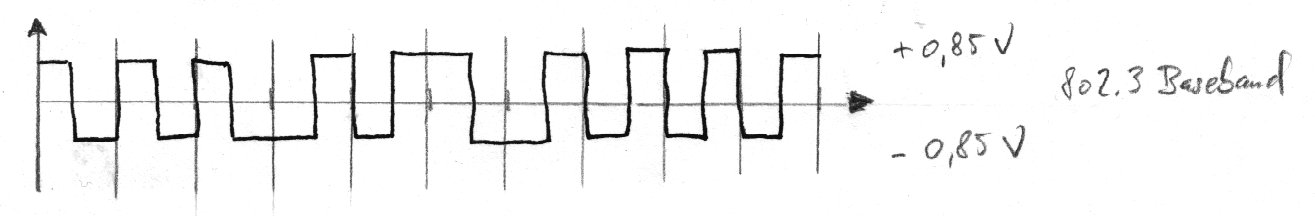
\includegraphics[width=\textwidth]{a3e5.jpg}

Manchester: \texttt{1} = zuerst vigh voltage, dann low, \texttt{0} = zuerst low voltage, dann hight\\
Differential Manchester: Umschalten am Anfang bedeutet \texttt{0}, kein Umschalten bedeutet \texttt{1}. In jeder Periode wird aber in der Mitte umgeschaltet zum Synchronisieren.\\
Beide brauchen doppelt so hohe Bandbreite, aber man kann schön synchronisieren.
\begin{enumerate}
\item Manchester: \texttt{1110010000}
\item Differential Manchester: \texttt{?001011000}
\item Das erste bit kann man nicht festlegen, weil die Spannung davor ja nicht bekannt ist.
\end{enumerate} 

\subsection*{Exercise 6: Data Encoding}
\texttt{0101110010}
\begin{enumerate}
\item Non-Return-to-Zero: \\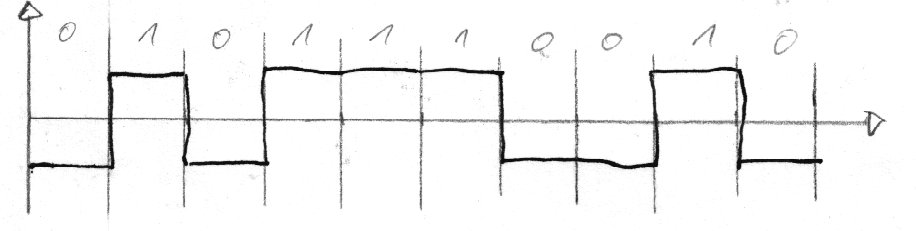
\includegraphics{a3e6_1.jpg}
\item Return-to-Zero:
\begin{itemize}
\item unipolar: \\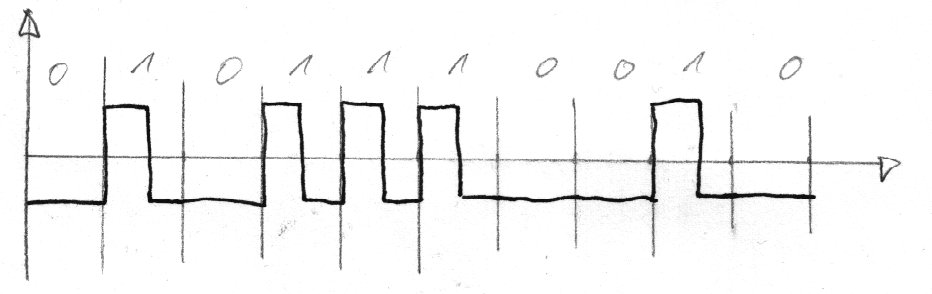
\includegraphics{a3e6_2a.jpg}
\item bipolar: \\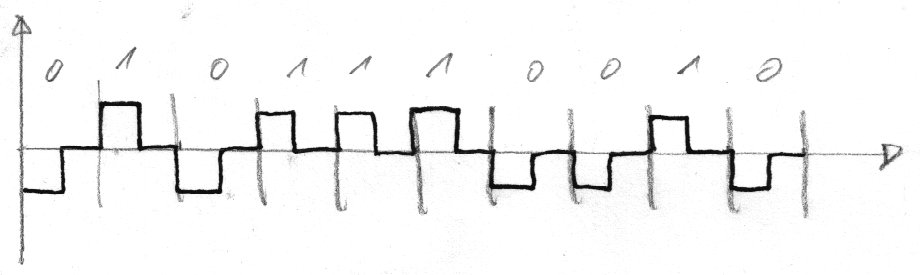
\includegraphics{a3e6_2b.jpg}
\end{itemize}
\item Differential Non-Return-to-Zero (NRZ Inverted; bei jeder \texttt{1} wechseln):\\ 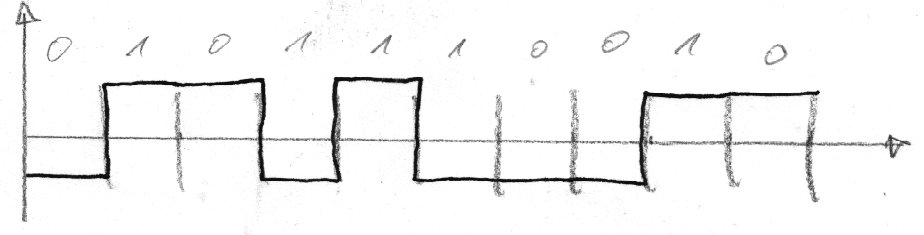
\includegraphics{a3e6_3.jpg}
\item Manchester: !! Nach IEEE 802.3 müßte man das anscheinend an der Zeitachse spiegeln !!\\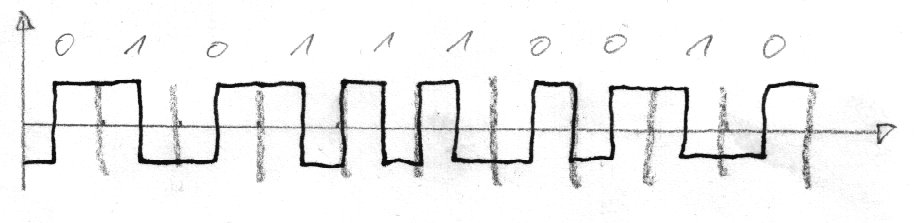
\includegraphics{a3e6_4.jpg}
\item Differential Manchester: \\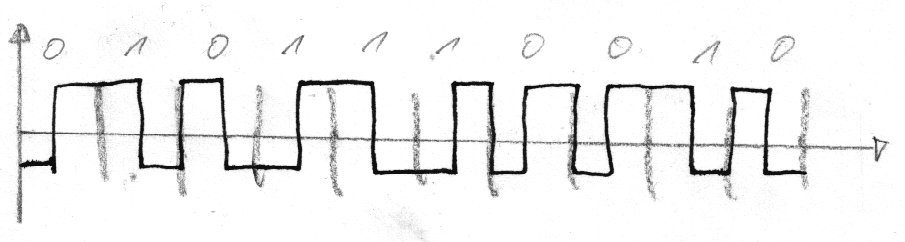
\includegraphics{a3e6_5.jpg}
\end{enumerate}

\subsection*{Exercise 7: Manchester Encoding \& Bandwidth}
Manchester braucht immer doppelt soviel Bandbreite. Abhilfe: B4B5-Kodierung etc. 

\subsection*{Exercise 8: Traditional Telephony vs. ISDN}
Telefon ist analog. ISDN (Integrated Services Digital Network) digital.\\
ISDN: Integration von Stimmen- und Nichtstimmenübertragung. Digital bit Pipe, bidirectional, mehrere Kanäle. NT-Box verbindet sich über Kupferkabel mit dem Abieter. 

\subsection*{Exercise 9: Modulation}
Bitsequenz: \texttt{000110010011}. Kombination aus Amplitude Shift Keying (ASK) und Differential Phase Shifting (Differential PSK).\\
\begin{enumerate}
\item
\begin{tabular}{|c|c|c|}
\hline Symbol & Amplitude & Phase Shift \\
\hline 00 & 1 & 0 \\ 
\hline 01 & 2 & 0 \\ 
\hline 10 & 1 & $\pi$ \\ 
\hline 11 & 2 & $\pi$ \\ 
\hline 
\end{tabular} \\
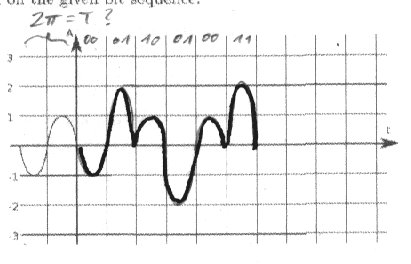
\includegraphics[scale=2]{a3e9_1.jpg}

\item
\begin{tabular}{|c|c|c|}
\hline Symbol & Amplitude & Phase Shift\\ 
\hline 000 & 1 & $0$ \\ 
\hline 001 & 2 & $0$ \\ 
\hline 010 & 1 & $\frac{\pi}{2}$ \\ 
\hline 011 & 2 & $\frac{\pi}{2}$ \\ 
\hline 100 & 1 & $\pi$ \\ 
\hline 101 & 2 & $\pi$ \\ 
\hline 110 & 1 & $\frac{3\pi}{2}$ \\ 
\hline 111 & 2 & $\frac{3\pi}{2}$ \\ 
\hline 
\end{tabular} \\
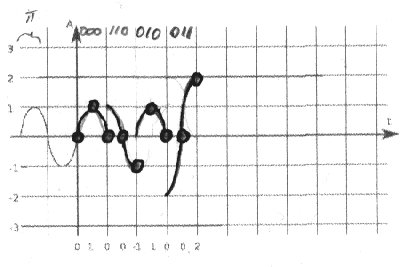
\includegraphics[scale=2]{a3e9_2.jpg}
\end{enumerate}

\subsection*{Exercise 10: Modulation 2}
\begin{tabular}{|c|c|c|}
\hline Symbol & Amplitude & Phase Shift \\ 
\hline 00 & 1 & $\pi$ \\ 
\hline 01 & 2 & $\pi$ \\ 
\hline 10 & 2 & 0 \\ 
\hline 11 & 1 & 0 \\ 
\hline 
\end{tabular} 

\subsection*{Exercise 11: Modulation 3}
Bitsequenz: \texttt{100101111001}. Frequenz- und Amplitudenverschiebung\\
\begin{tabular}{|c|c|c|}
\hline Symbol & Frequenz & Amplitude \\ 
\hline 00 & f & 1 \\ 
\hline 01 & f & 2 \\ 
\hline 10 & 2f & 1 \\ 
\hline 11 & 2f & 2 \\ 
\hline 
\end{tabular} \\
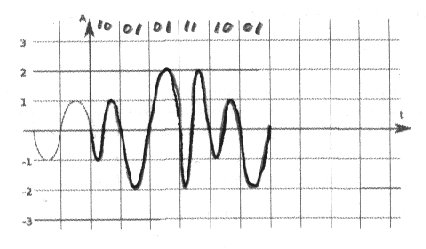
\includegraphics[scale=2]{a3e11.jpg}

\section*{Assignment 4}

\subsection*{Exercise 1: Cyclic Redundancy Checksum}
$x^4+x+1$ wird repräsentiert durch \texttt{1011}. ($G(x)$) \\
Binäre Addition und Subtraktion sind wie \texttt{XOR}, ohne Übertrag. Man macht jetzt einfach Polynomdivision und guckt, was übrigbleibt (im Optimalfall 0).\\
Wenn ein Fehler in der Übertragung von $T(x)$ auftritt, kommt $T(x)+E(x)$ an. Jedes \texttt{1}-Bit in $E(x)$ zeigt ein umgekipptes Bit in $T(x)$ an. Weil $T(x)/G(x)$ ja \texttt{0} ist, ist bei einer fehlerhaften Übertragung der Rest also $E(x)/G(x)$.\\
Wenn in $E(x)$ eine \texttt{1} vorkommt, kann $G(x)$, sofern dieses mehr als einen Term ($x^y$) enthält, nicht teilen. Der Fehler wird also entdeckt.\\
Wenn in $E(x)$ zwei \texttt{1} vorkommen, ist $E(x)=x^j+x^i$. Das kann man auch als $E(x)=x^j(x^{i-j}+1)$ schreiben. Solange $G(x)$ also nicht durch $x$ oder $x^k+1$ teilbar ist, wird der Fehler erkannt.
\begin{enumerate}
\item \texttt{011101100010}\\
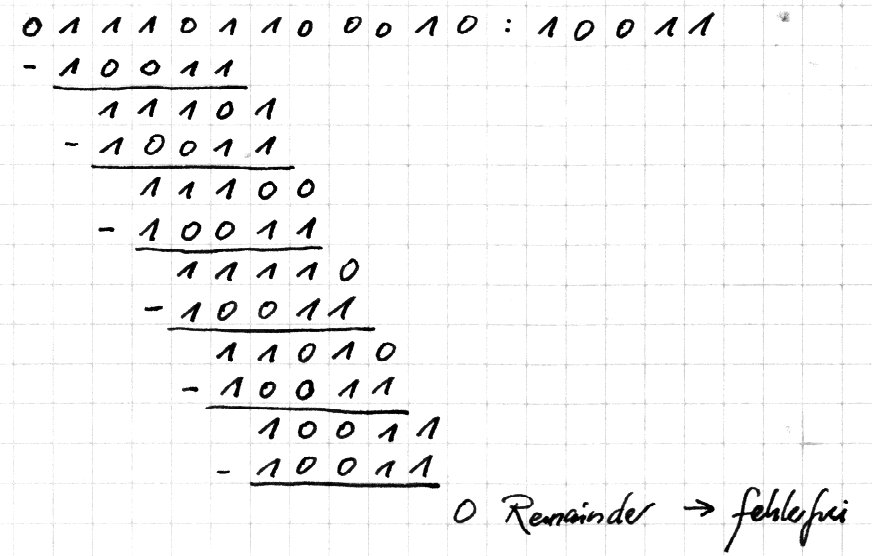
\includegraphics{a4e1_1.jpg}
\item \texttt{010100101001}\\
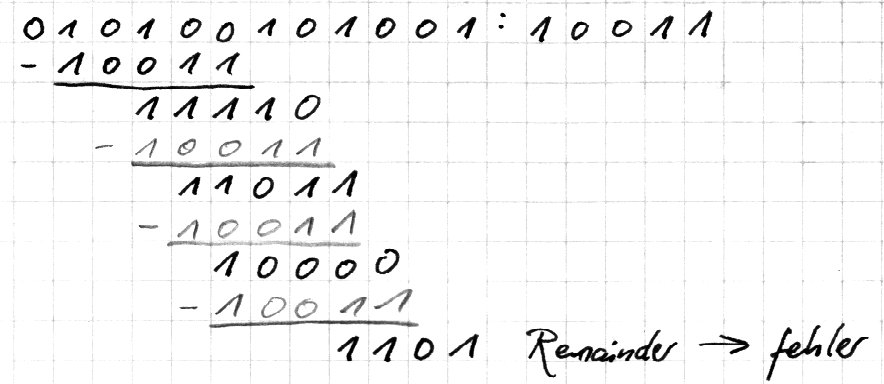
\includegraphics{a4e1_2.jpg}\\
Da offenbar ein Fehler vorliegt, rechnen wir nochmal die Prüfsumme aus. Dazu überschreiben wir die Prüfsumme mit Nullen. Die Prüfsumme ist so lang wie der Grad des Prüfpolynom $x^4+x+1$, also vier Bit.\\
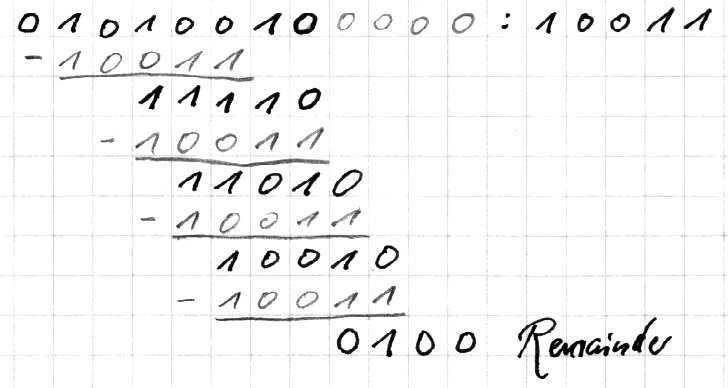
\includegraphics{a4e1_2b.jpg}\\
\item \texttt{111101101100}\\
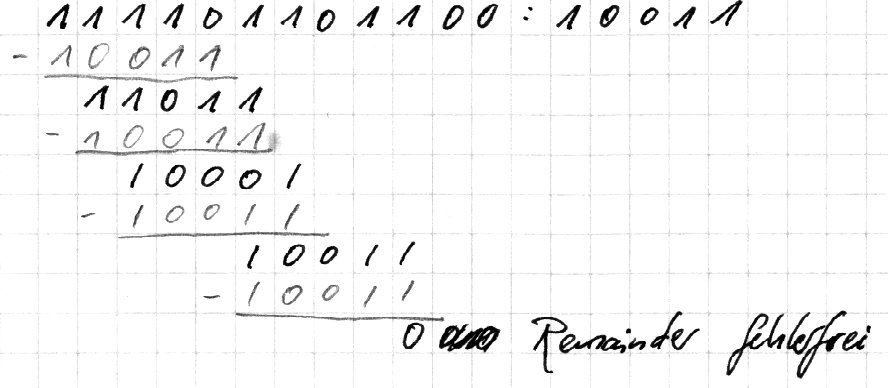
\includegraphics{a4e1_3.jpg}
\end{enumerate}

\subsection*{Exercise 2: Transmission with HDLC}
High Level Data Link Control\\

\begin{tabular}{|c|c|c|c|c|c|}
\hline 8 Bit & 8 & 8 & $\geq0$ & 16 & 8 \\ 
\hline \texttt{01111110} & Adress & Control & Data & Checksum & \texttt{01111110} \\ 
\hline 
\end{tabular} \\
\begin{tabular}{|c|c|c|c|}
\hline 1 Bit & 3 & 1 & 3 \\ 
\hline 0 & Seq & P/F & Next \\ 
\hline 0 & 011 & 0 & 010 \\
\hline 
\end{tabular} 
Type 0: Information\\
Seq: 3-Bit Sliding Window Sequenznummer. In diesem Fall 3 (das nächste Frame). (\texttt{011})\\
P/F: 0 (egal)\\
Next (piggybacked ACK): Acknowledgement für Frame 2 (\texttt{010})\\
\begin{enumerate}
\item Bitsequenz \texttt{110111110101}. Polynom $G(x)=x^4+x+1$.\\
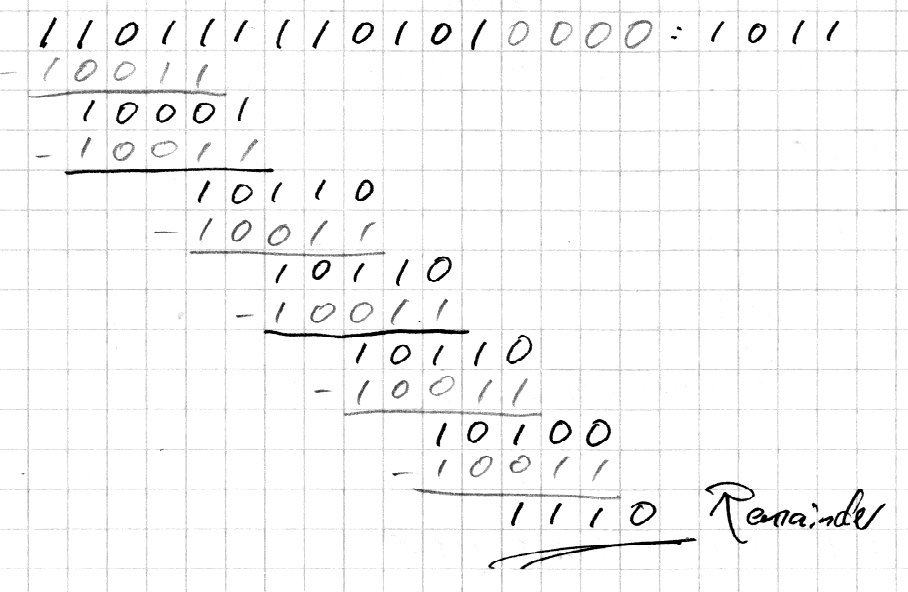
\includegraphics{a4e2_1.jpg}\\
Checksumme ist \texttt{1011}.
\item 
\begin{tabular}{|c|c|c|c|c|c|}
\hline \ldots & Address & Control & Data & Checksum & \ldots \\ 
\hline \texttt{01111110} & \texttt{1111}\textbf{0}\texttt{111} & \texttt{0 011 0 010} & \texttt{11011111}\textbf{0}\texttt{0101} & \texttt{1011} & \texttt{01111110} \\ 
\hline 
\end{tabular} \textbf{Fett}: Bitstuffing!!! Nach fünf einsen muß ne null kommen.
\item 
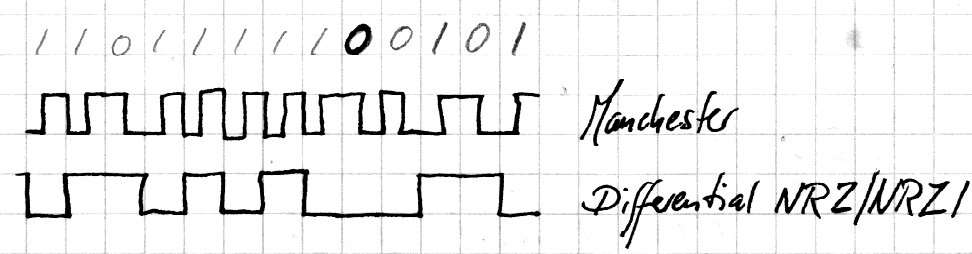
\includegraphics{a4e2_3.jpg} Invertiert wegen IEEE 802.3
\end{enumerate}

\subsection*{Exercise 3: Transmission Capacity}
Window Size $W=7$. Frame Size $1500$ Bytes. Round Trip Time = 50 ms.\\
Host kann $7 \cdot 1500 = 10500$ Bytes senden, ohne ein ACK zu bekommen. Weil RTT 50 ms ist, ist nach 50 ms ein ACK da und das Fenster kann verschoben werden. In einer Sekunde kann der Host 20 ACKS bekommen (1000/50 ms). Also können $20\cdot 10500=210000$ Bytes/s verschickt werden, das sind ungefähr 1.6 Mbps.

\subsection*{Exercise 4: Sliding Window Mechanism}
Sliding Window: Jedes ausgehende Frame enthält eine \textbf{Sequenznummer} von 0 bis $2^n-1$. Der Sender hat ein Set von Sequenznummern der Frames, die er senden darf. Der \textbf{Empfänger} hat ein Set von Sequenznummern, die er emfangen darf.\\
Bekommt der Sender ein Frame von seinem Network Layer, bekommt das die höchste Sequenznummer, und die obere Grenze des Fensters geht um 1 hoch, solange die Fenstergröße nicht das Maximum überschreitet. Wenn er ein Acknowledgement vom Emfpänger bekommt, geht die untere Grenze eins hoch.\\
Der \textbf{Empfänger} nimmt nur die Frames an, deren Sequenznummer innerhalb seines Fensters sind. Wenn die Sequenznummer aber dem unteren Rahmen des Fensters entspricht, sendet er sein Acknowledgement und rotiert das Fenster um 1 weiter. Die Fenstergröße bleibt also immer gleich. Die Reihenfolge, in der die Frames ankommen, ist egal, außer die Fenstergröße ist 1. \\

Bei einem 50 kbps Kanal mit einer 500 ms round trip time, auf dem 1000 bit große Frames gesendet werden sollen, ist eine sinnvolle Fenstergröße 26: Um ein Frame in die Leitung zu pumpen, braucht der Sender $50 \frac{kbit}{s}\cdot 1 kbit = 50 \frac{1}{s} = 20 s$. Nach $20+(\frac{500 ms}{2})=270 ms$ ist das Frame beim Empfänger angekommen angekommen, und nach $270+(\frac{500 ms}{2}) = 270+250 ms = 520 ms$ ist das Acknowledgment da. In der Zeit kann der Sender aber $520ms /20 ms = 26$ Frames raushauen. Wenn das Fenster die Größe 26 hätte, würde grade nach dem 26. Frame das erste bestätigt werden und der Sender könnte das Fenster verschieben. \\

Wenn dabei allerdings irgendeins der Frames kaputtgeht, bekommt das der Sender ja erst mit, nachdem ganz viele aufeinanderfolgende Frames schon gesendet wurden. Der Empfänger sitzt dann da mit einem fehlenden Frame mittendrin und kann die Framesequenz nicht an die Network Layer weitergeben. Schön blöd.\\
Zwei Möglichkeiten: entweder \textbf{go back n}, also einfach alle Frames nach dem kaputten verwerfen und keine Acknowledgements dafür senden. (Das ist, also ob das Empfänger-Fenster die Größe 1 hätte). Beim Sender gehts dann irgendwann nicht weiter, weil das Acknowledgement fürs kaputte Frame fehlt. Deshalb gibts da nen timeout, und das kaputte Frame (das erste im Senderfenster) wird nochmal gesendet. Das kann viel Bandbreite verschwenden\\
Oder man macht \textbf{selective repeat} und behält die nachfolgenden heilen Frames. Der Sender bekommt dann irgendwann mit, daß eins fehlt, und schickt nur das nochmal, macht ansonsten aber weiter wie gehabt. Das kann hohen Speicherverbruch beim Empfänger nach sich ziehen, weil die Frames ja zwischengespeichert werden, bis das kaputte Frame da ist und zusammen mit den nachfolgenden an die Network Layer gegenben werden kann.\\
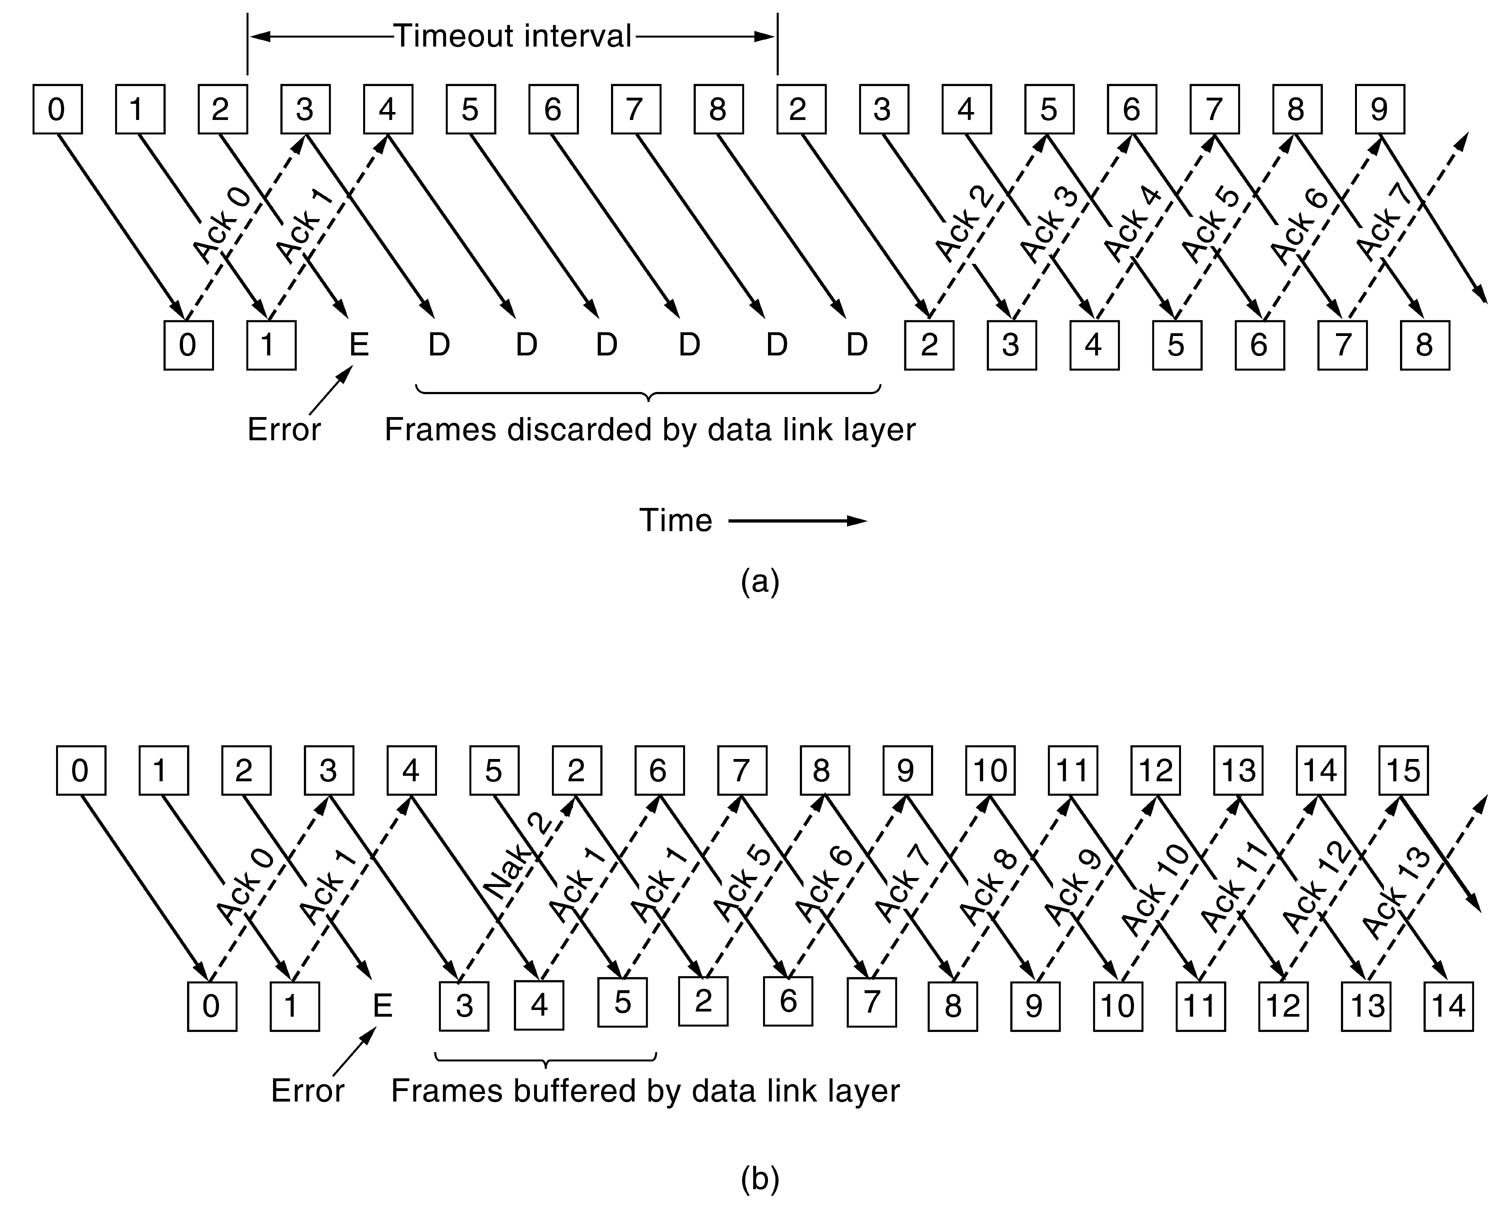
\includegraphics[width=\textwidth]{a4e4.jpg}\\

HDLC: Jedes Frame enthält Sequenznummer N(S) und Acknowledgenummer N(R). N(R) bestätigt alle Frames bis R-1, also wird als nächstes R erwartet. R wird mit M modulo gerechnet, damit der Counter nicht überläuft. \\
\begin{enumerate}
\item Die maximale Fenstergröße W ist dann M-1.
\item Wenn M=8 ist und die Fenstergröße W=7, und die Frames mit N(S)=5,6,7,0,1 gesendet wurden, können die Frames mit den Sequenznummern 2 und 3 gesendet werden, bevor ein Acknowledgement kommt. (M - 1 =7; 5 Frames gesendet $\Rightarrow$ letzte Sequenznummer + 1,2)\\
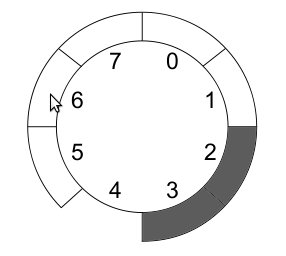
\includegraphics[width=.3\textwidth]{a4e4_2.jpg}
\item Wenn 5,6,7,0,1 gesendet wurden und folgende Acknowledgements kommen: 

\begin{enumerate}
\item N(R)=2: bestätigt sind 5,6,7,0,1. Fenster: 2,3,4,5,6,7,0.\\
\includegraphics[width=.8\textwidth]{a4e4_3a.png}
\item N(R)=6: bestätigt ist 5. Fenster: 2,3,4\\
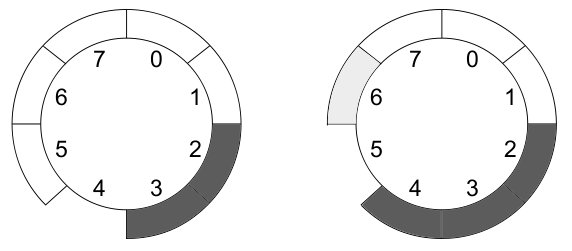
\includegraphics[width=.8\textwidth]{a4e4_3b.jpg}
\item N(R)=5: bestätigt ist 4. Fenster: 2,3.\\
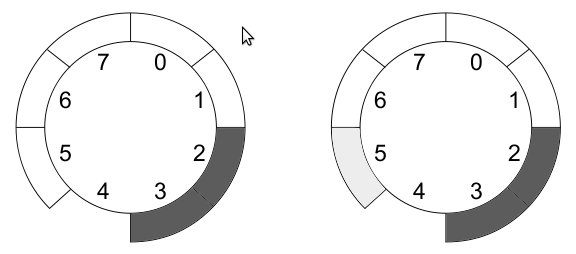
\includegraphics[width=.8\textwidth]{a4e4_3c.jpg}
Die Frames mit den Sequenznummern 2 und 3 sind beim Sender schon in das Fenster geschaufelt und möchten gern gesendet werden. Jetzt kommt die bestätigung N(R)=5, also daß Frame 4 beim Empfänger ist. 
\end{enumerate}

\end{enumerate}



\subsection*{Exercise 5: Network Topologies}
Durchschnittliche Länge der Pfade: $ \frac{1}{\mathrm{alle zu erreichenden Knoten}} \sum_{i=1}^{\mathrm{laengstmoeglicher Pfad}}{i} $.

\subsection*{Exercise 6: Network Topologies 2}
\begin{itemize}
\item Bus: Alle teilen sich ein Kabel, jeder kann sich einfach ohne Authentifizierung dranhängen, kann komplett zusammenbrechen wenn das Kabel ein Problem hat
\item Star: zentaler Hub, Anzahl der Knoten ist begrenzt, Hub kann bottleneck sein...
\end{itemize}

\subsection*{Exercise 7: Introduction to Wireshark}


\section*{Assignment 5}

\subsection*{Exercise 1: LLC vs. MAC}
\begin{itemize}
\item LLC (Logical Link Control): bietet der Network Layer eine einheitliche Schnittstelle zu den verschiedenen 802-Protokollen. Kümmert sich außerdem um Fehler- und Flußkontrolle (Seq, Ack). LLC-Header und -Paket werden im von MAC in einem 802.x Frame übertragen (sind Payload).
\item MAC (Media Access Protokoll): Implementiert verschiedene Übertragungstechnologien. Kümmert sich um Multi-Access auf Medium.
\end{itemize}

\subsection*{Exercise 2: Flow Control}
\begin{itemize}
\item Stop-and-Wait Protocol: Lange Untätigkeit, weil auf ACKs gewartet wird. Keine Parallelität.
\item Sliding Window Protocol: Kann abhängig von der Fenstergröße fortlaufend senden. Braucht u.U. nen großen Buffer. Wie geht man bei Übertragungsfehlern mit den korrekten Frames um? (Die Network Layer will die ja nur in der richtigen Reihenfolge)?
\begin{itemize}
\item Go-Back-n: Empfängerfenstergröße 1. Sender muß alle Frames nach dem kaputten wiederholen.
\item Selective Repeat: Großer Buffer. Der Sender muß nur das kaputte Frame nochmal senden.
\end{itemize}
\end{itemize}

\subsection*{Exercise 3: Sliding Window}
Ohne Vollduplex gibts nur teilweise Parallelität.

\subsection*{Exercise 4: The End-to-End Argument}

\section*{Assignment 6}

\subsection*{Exercise 1: Multiplexing and Multiple Access}
\begin{itemize}
\item Multiplexing: Multiplexer bündelt mehrere Signale und sendet sie über Übertragungsweg an Demultiplexer
\begin{itemize}
\item Time Division Multiplexing: Jeder sendet abwechselnd zu festgelegter Zeit (synchrones M.) bzw. wenn nötig. (mit Kanalkennung; asynchrones M.)
\item Frequency-Division Multiplexing: Jedes Signal eigene Trägerfrequenz
\item Wavelength-Division Multiplexing: Glasfaser; Jedes Signal eigene Trägerlichtfrequenz
\item Space-Division Multiplexing: Mehrere Kabel
\item Code-Division Multiplexing: Alle Signale unterschiedlich codiert (UMTS, PCI, KfZ-Zentralverriegelung...)
\end{itemize}
\item Multiple Access: Mehrere Teilnehmer haben Zugriff auf das Übertragungsmedium und teilen es sich (MAC-Protokolle)
\begin{itemize}
\item Time Division \ldots
\item \ldots
\end{itemize}
\item Duplex: Zwei Teilnehmer senden "`gleichzeitig"' auf verbindendem Übertragungsmedium \ldots
\begin{itemize}
\item TDM: halbduplex
\item FDM: duplex
\end{itemize}
\end{itemize}

\subsection*{Exercise 2: Media Access}
Carrier Sense: horcht ob Leitung belegt ist.\\
Statisch vs. dynamisch, Kollisionen vs. kollisionsfrei, fair vs. unfair Zugriffwahrsch. \ldots\\
Contention system: system in dem es zu Konflikten (Kollisionen) kommen kann\\

\textbf{pure ALOHA:} Alle senden, wenn sie was zu senden haben und horchen dann, ob es zu Kollisionen kommt. Wenn ja, wartet der Sender eine zufällige Zeit lang und sendet neu. Frames haben einheitliche Länge.\\
\textbf{slotted ALOHA:} Diskrete Intervalle, in die jeweils ein Frame paßt. Muß natürlich synchronisiert werden. \\

\textbf{Carrier Sense Multiple Access Protocols:} Stationen lauschen an der Leitung und verhalten sich entsprechend.
\begin{itemize}
\item \textbf{1-persistent:} Station überträgt Frame mit der Wahrscheinlichkeit 1 wenn die Leitung frei ist, und wartet zufällig lange, wenn es dabei zur Kollision kommt.
\item \textbf{Nicht-persistent:} Wenn die Leitung belegt ist, wartet die Station eine zufällige Zeit und horcht erst dann wieder.
\item \textbf{n-persistent:} Slotted Channels. Wenn Leitung (Slot) frei ist, sendet Station mit Wahrscheinlichkeit $p$. Wenn es nicht zum Senden kommt, sondern irgendwann eine andere Station sendet, wird zufällig lange gewartet. Ist die Leitung ursprünlich belegt, wird auf den nächsten Slot gewartet. 
\end{itemize}

\textbf{CSMA mit Collision Detection:} Kollision wird erkannt, indem das gesendete Signal mit dem gehörten verglichen wird. Das wird gemacht, wenn ein Frame übertragen wurde. Dann checken die anderen, ob die Leutung frei ist (Contention period). $\tau$ ist die Zeit, die ein Signal braucht um den Weg zwischen den zwei am weitesten voneinander entfernten Stationen zurückzulegen. Eine Station kann erst sicher sein, sich den Kanal gesichert zu haben, wenn sie $2\tau$ lang von keiner Kollision gehört hat, weil die entfernteste Station ja anfangen kann zu senden, kurz bevor das Signal ankommt. Kollisionserkennung läuft analog. MAC garantiert keine verläßliche Übertragung.\\
\textbf{Kollisionsfreie Protokolle:} Bei CSMA/CD können immer noch Kollisionen in der Contention period auftreten. Das ist bei langen Kabeln (großen $\tau$) und kleinen Frames doof. Kollisionsfreie Protokolle sind ineffizient bei wenig Traffic, bei solchen mit Kollision ist das umgekehrt.
\begin{itemize}
\item \textbf{Bit-Map Protokoll:} Contention period (Bitmap) besteht aus genauso vielen Slots wie es Stationen gibt ($N$). Wenn Station $j$ was zu senden hat, sendet sie eine eins in Slot $j$. Wenn die Contention period vorbei ist, wissen also alle, wer was senden will. Die Stationen senden dann nacheinander (reservation protocols). Das ist unfair gegenüber den Stationen mit kleinem $j$, weil die durchschnittlich länger warten müssen. Bei wenig Traffic ist außerdem der Overhead hoch, weil vor einem einsamen Frame ja immer noch die Bitmap kommt. 
\item \textbf{Binary Countdown:} Stationen die senden wollen schicken ihre Adresse binärcodiert. Bekommen sie mit, daß eine Station, die eine höherwetige Null von ihnen mit einer eins überschreibt, also auch senden will, geben sie auf. Wenn \texttt{0010}, \texttt{0100}, \texttt{1001} und \texttt{1010} senden wollen, geben \texttt{0010} und \texttt{0100} auf, aber  \texttt{1001} und \texttt{1010} machen erstmal weiter, bis \texttt{1001} merkt, daß \texttt{1010} eine ihrer Nullen überschrieben hat. Die Station mit der höchsten Adresse gewinnt also. 
\end{itemize}

\textbf{Limited-Contention-Protokolle}: Bei wenig Traffic wär es gut, konkurrierende Multi-Access-Techniken einzusetzen, bei viel Traffic aber lieber kollisionsfreie. Konkurrierende Stationen versuchen ja mit der Wahrscheinlichkeit $p$, den Channel zu bekommen. Bei weniger Stationen steigt die Wahrscheinlichkeit, daß sie den Channel bekommen. In Limited-Contention-Protokollen werden mehrere Stationen zu Gruppen zusammengefaßt, die dann untereinander um einen bestimmten Slot konkurrieren.
\begin{itemize}
\item \textbf{Adaptive Tree Walr Protocol:} Alle Stationen sind Blätter eines binären Baumes. Jeder Slot ist einem Teilbaum zugeordnet. Wenn es da zu Kollisionen kommt, wird Tiefensuche gemacht, bis die Stationen gefunden sind die senden wollen.
\end{itemize}

\subsection*{Exercise 3: Scaling of Token Ring}
Ein Token Ring besteht aus verketteten Stationen, die einfach in die Leitung kopieren was sie empfangen. Wenn alle Stationen untätig sind, wird das \textbf{Token} rumgereicht. Bekommt eine Station, die was senden will, dieses 3-Byte-Token, ersetzt sie es durch ihr Frame. Wenn das einmal durch den Ring gegangen ist, nimmt die Station es wieder raus. Die Station die das Frame empfangen soll, schreibt einfach ein Acknowledgement-Bit rein. Token Ring ist in IEEE 802.5 definiert und betrifft Physical Layer und Data Link Layer. \\

Frames: 
\begin{itemize}
\item Token: 
\begin{tabular}{|c|c|c|}
1 Byte & 1 & 1\\
\hline Starting Delimiter & Access Control & Ending Delimiter \\ 
\hline 
\end{tabular} 
\item Data:
\begin{tabular}{|c|c|c|c|c|c|c|c|c|}
 1 Byte & 1 & 1 & 2 or 6 & 2 or 6 & unbegr. & 4 & 1 & 1 \\ 
\hline SD & AC & FC & Dest Addr & Source Addr & Data & Checksum & ED & FS \\ 
\hline 
\end{tabular} 
FC: Frame Control, FS: Frame Status
\end{itemize}
Start und Ending Delimiter werden anhand von ungültigem Differential Manchester erkannt. Durch das Kippen eines Bits im ED wird das Token zum Anfang eines Frames.

\subsection*{Exercise 4: Efficiency of Token Ring}
Effizient bei hoher Auslastung. Außerdem fairer Medium Access (wegen Token). Bei geringer Auslastung nicht so pralle. 

\section*{Assignment 7}

\subsection*{Frame Size}
Ein 10 MBit/s CSMA/CD LAN hat einen Bus mit 50m Länge. Die Geschwindigkeit des Signals ist $2\cdot 10^8$m/s.
\begin{enumerate}
\item Wie lang dauert die Kollisionserkennung maximal?\\
Weil es sein kann, daß die zweite Station in dem Moment anfängt zu senden, indem das Signal der ersten Station ankommt. Bis die erste Station davon erfährt, vergeht zweimal die Zeit, die das Signal von A zu B braucht. Also: $2\cdot \frac{50m}{2\cdot 10^8\frac{m}{s}} = 5\cdot 10^{-7}s$.
\item Damit die Stationen auch wirklich mitbekommen, daß es ne Kollision gab, müssen die Frames also mindestens so lange für die Übertragungs brauchen. \\
Also $ \frac{framelength}{capacity}\>5 \cdot 10^{-7}s $\\
$ \frac{framelength}{capacity} > 10 \frac{Mbit}{s}\cdot 5 \cdot 10^{-7}s = 5 Bit $ 
\end{enumerate}

\subsection*{FDDI Performance}
100 Stationen sind in einem Ring. Die Umlaufzeit des Tokens ist 40 ms und jede Station darf das Token 10 ms lang behalten. Maximale Effizienz?\\
\\
Das Token ist insgesamt $100\cdot 10ms+40ms$ in Beschlag. Wenn die Stationen unendlich viel Daten zu senden haben und während sie das Token haben, ununterbrochen senden, ist die Effizienz $ \frac{1000}{1040} = 0.96$.

\subsection*{ATM}

\subsection*{•}


\section*{Important Stuff}

\subsection*{IP-Header}
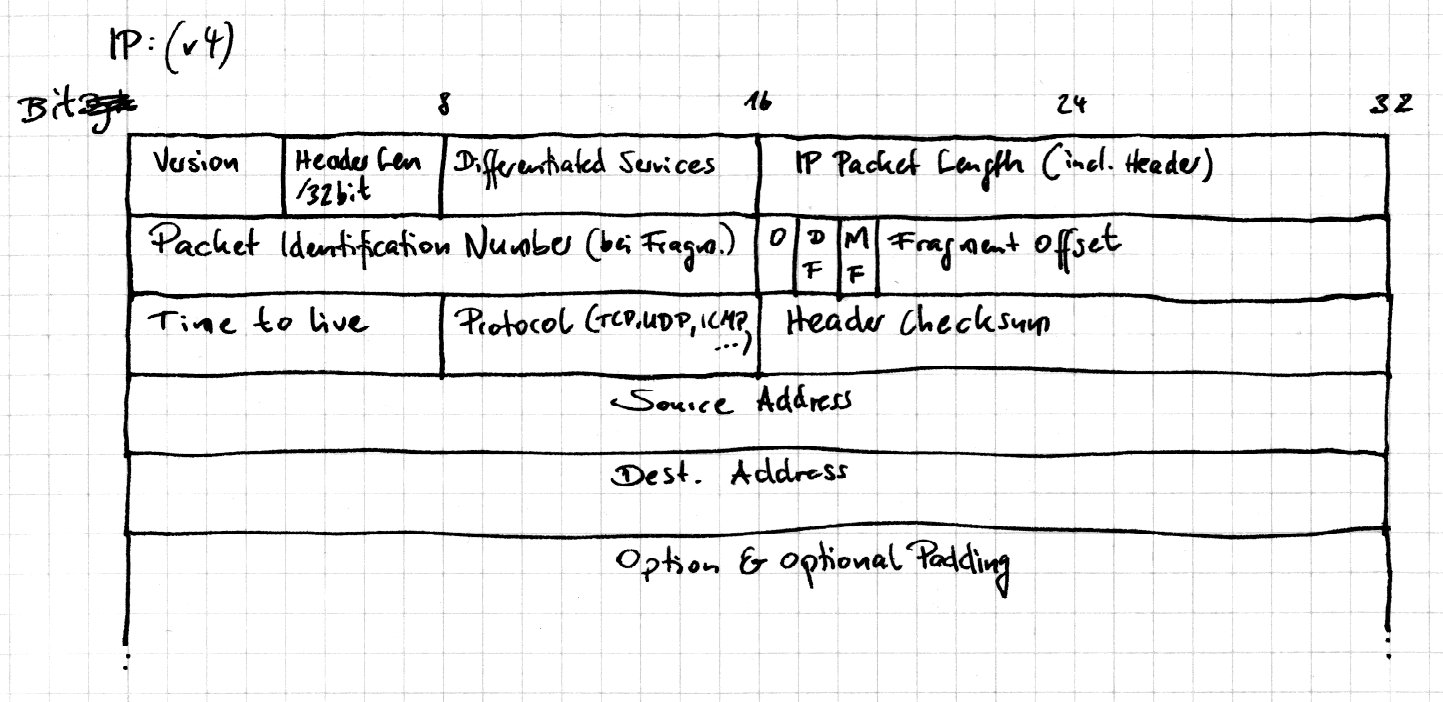
\includegraphics[width=\textwidth]{ipheader.jpg}
\begin{itemize}
\item Version: Bei IPv4 immer \texttt{0100}
\item Header Len: Länge des Headers als Vielfaches von 32 Bit. Meistens \texttt{0101}, hängt von der Menge der Optionen ab
\item Differentiated Service Service - Type of Service: Wie Traffic Class bei IPv6
\item IP Packet Length: Gesamtlänge des Pakets in Byte, inkl. Header (max. $65535$)
\item Packet Identification: Gemeinsamer Index für fragmentierte Pakete; Wenn ein Paket zu groß für die Data Link Layer ist, wird es zerlegt. 
\item Don't Fragment Bit: Paket darf nicht fragmentiert werden. Wenn es irgendwo zu lang ist, wird eine ICMP-Fehlernachricht an die Quelle gesendet.
\item More Fragment Bit: Es folgen noch weitere Fragmente mit demselben Index
\item Fragment Offset: Offset des Fragments relativ zum Anfang des Paketes, Vielfaches von 8 Bytes
\item Time to live: Eigentlich Hop Count
\item Protocol: Das von diesem Paket transportierte Protokoll (ICMP,TCP,UDP,$\ldots$)
\item Header Checksum: Header wird in 16-Bit-Sequenzen aufgeteilt, die werden nach Einerkomplement addiert und zum Schluß wird das invertiert. Muß bei jedem Hop neu berechnet werden.
\item Source Address: Quelladresse
\item Destination Address: Kann Einzelknotenadresse, Mehrfachknotenadresse (Multicast) oder Sammeladresse (Broadcast) sein
\item Options: z.B. Strict Source Routing (fester Pfad), Record Route (jeder Router hängt seine IP-Adresse ran), Timestamp (Jeder Router hängt Zeit ran),\ldots
\end{itemize}

\subsection*{TCP}
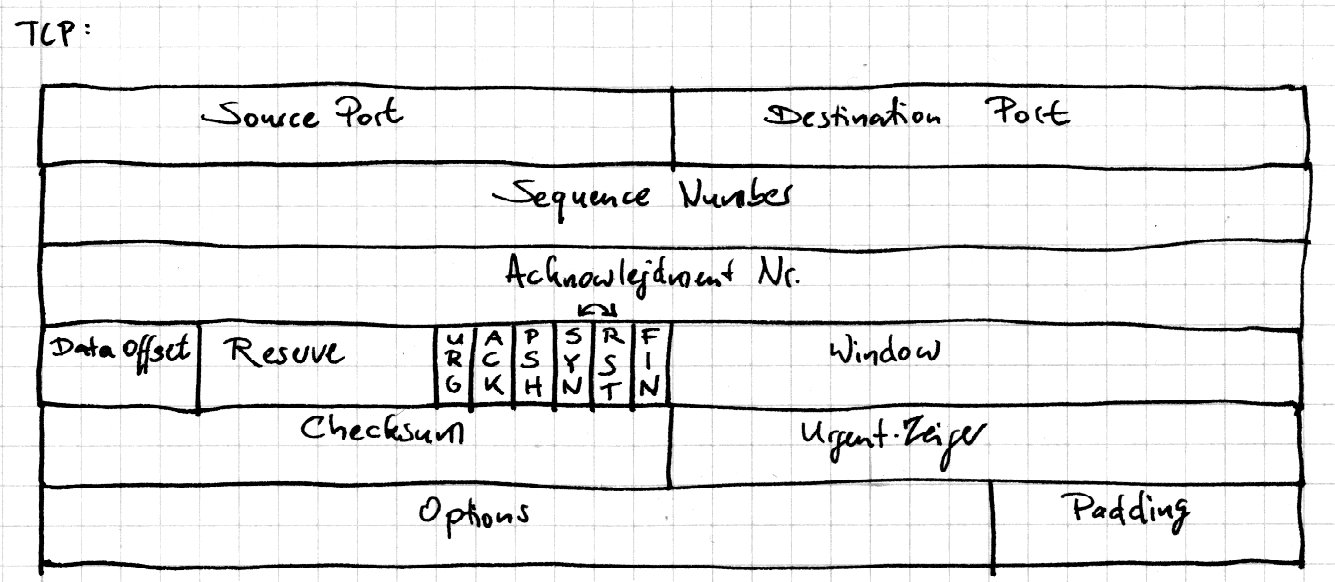
\includegraphics[width=\textwidth]{tcpheader.jpg}
\begin{itemize}
\item Data Offset: die Position an der der Datenteil losgeht in Words
\item URG: Urgent Pointer ist an
\item ACK: Segment ist Acknowledgement.
\item PSH: Pushed Data: Der Empfänger soll die Daten bitte gleich weitergeben und nicht erst buffern.
\item RST: Reset
\item SYN: Um Verbindungen auszubauen. Mit ACK aus: connection request, mit ACK an: connection accepted
\item FIN: schließt verbindung
\item Window Size: Fenstergröße im Sliding Window
\item Checksum: Prüfsumme über das komplette Segment. Berechnet wie bei IP.
\item Urgent Pointer: Wo im diesem Segment eilende Daten anfangen
\item Options: z.B. wieviel Payload ein Host bereit ist zu empfangen. 
\end{itemize}

TCP kümmert sich um Timeout, Neuversendung und darum, die ankommenden Pakete in die richtige Reihenfolge zu bringen, weil IP das nicht macht. Socketnummer: IP-Adresse+16 bit Port (bis 256: reserviert). Es können mehrere Verbindungen auf dem selben Socket laufen. TCP-Verbindungen sind vollduplex und point-to-point. Kein Multi- oder Broadcasting. Die TCP-Segmente (in die TCP seine Byteströme aufteilt), sind in ihrer Größe begrenzt vom IP-Payload (63,535 byte) und der Maximum Transfer Unit (MTU) des Netzwerks. Der Header ist 20 Bytes groß. TCP kann also maximal $63535-20-20$ Bytes Daten im Segment haben. TCP nutzt Sliding Window: im ACK steht die Seg Nr. die als nächstes erwartet wird. 


\begin{itemize}
\item  protocol (defintion)
\item  seriell vs. parallel
\item  multiplexing
\item  overhearing, eavesdropping, etc
\item  cross layering
\item  unacknowledged vs acknowledged
\item  push vs. pull
\item  LAN, MAN, WAN
\end{itemize}


\end{document}
